\documentclass{article}
\usepackage{ctex}
\usepackage{enumerate}
\usepackage{graphicx}
\usepackage{setspace}
\usepackage{multirow}
\usepackage{amsmath}

\begin{document}
    \setstretch{1.2} 
    \zihao{5}
    \section*{基于支持向量机与神经网络的中小微企业信贷策略}
    \begin{center}
        \textbf{概述}    
    \end{center}\par
    如何制定针对中小微企业的\textbf{信贷策略}从而达到利益最大化对银行来
    说是至关重要的。本文使用\textbf{聚类分析}、\textbf{支持向量机}、\textbf{对应分析}及\textbf{BP
    神经网络}等方法,通过对所给企业进行行业分类,借助于 MATLAB、
    R 统计分析软件、Python 及 SPSS 等工具,针对附件中所给数据,
    比较准确的给出银行对于各企业是否放贷、贷款额度、利率及期限等
    相关信贷策略。针对问题一,通过对附件一数据进行处理:
    \begin{enumerate}
        \item 删除信誉评级为 D 的企业;
        \item 剩余企业按照 A、B、C 三个等级进行分组;
        \item 计算企业总盈利额;
        \item 是否违约;
    \end{enumerate}\par
    按照 A、B、C 三类企业使用聚类分析进行分组,在三类企业中再
分别分出优、良两类企业,共计六类企业,相应信贷策略在正文(表 5)及支撑材
料(表问题一)中明确给出。\par
针对问题二,通过使用支持向量机找出能够区分全部企业盈利额数据点的最优
超平面,将企业分为优、良两个等级。具体信贷策略及一亿元的详细分法等相关
数据见正文(表 8)及支撑材料(表问题二)。\par
针对问题三,主要考虑新型冠状病毒对企业盈利额的负面作用,同时为消除数
量量纲对后续计算产生的影响,将企业盈利额从 2019 年 1 月 1 日到 2 月 21 日数
据与 2020 年 1 月 1 日到 2 月 21 日数据作为新冠爆发前与新冠爆发后数据,见支
撑材料(表问题三),即每个企业对应两个数据,使用对应分析找出受新冠影响
较大与较小的企业。对这些企业给出更改过后的信贷策略,详见正文部分(表 9
及表 10)。\par
另外,针对上述三个问题给出误差分析。为改进问题二、三中所使用的模型,
通过 BP 神经网络预测附件二中企业信誉评级与是否违约的情况,将附件一中企业
盈利额、客户流失率、信誉评级以及是否违约作为训练集,附件二中企业盈利额、
客户流失率作为测试集进行测试,最终测试结果见支撑材料(模型改进),并根
据测试结果给出相应的信贷策略,见正文(表 11)。最后给出模型的评价及推广。
\\\\\\
\textbf{关键字:信贷策略 聚类分析 支持向量机 BP神经网络 对应分析}\newpage
\section{问题的提出}
\subsection{基本情况}
2014 年 9 月 17 日,国务院总理李克强提出进一步扶持小微企业发展推动大众
创业万众创新,他在会议中明确指出,小微企业是发展的生力军、就业的主渠道、
创新的重要源泉。加大对小微企业、个体工商户特别是在改革中“呱呱坠地”新
生者的扶持,让它们在公平竞争中搏击壮大,可形成示范效应,推动大众创业、
万众创新,也能增添社会活力和发展内生动力,促进经济稳定增长和民生改善[1]。
各行各业积极配合,特别是国有大型银行及地方控股银行。\par
目前,银行如何确定是否放贷及贷款额度、利率和期限等信贷策略成为全部中
小企业首要关注的问题。
\subsection{问题提出}
某银行对确定要放贷企业的贷款额度为 10~100 万元;年利率为 4\%~15\%;贷款
期限为 1 年。根据三个附件给出的数据建立数学模型,研究对中小微企业的信贷
策略,主要解决下列三个问题:
\begin{itemize}
    \item [*] 对附件 1 中给出的 123 家企业的基本信息、进项与销项发票信息进行分
    析,给出该银行在年度信贷总额固定时对这些企业的信贷策略。
    \item [*] 在问题 1 的基础上,对附件 2 中 302 家企业的相关信息进行数据分析,
    给出该银行在年度信贷总额为 1 亿元时对这些企业的信贷策略。
    \item [*] 由于企业的生产经营和经济效益可能会受到一些突发因素影响,而且突
    发因素往往对不同行业、不同类别的企业会有不同的影响。因此结合突发因素所
    带来的影响给出该银行在年度信贷总额为 1 亿元时的信贷调整策略。
\end{itemize}
\section{问题的分析}
\subsection{背景分析}
    目前国内中小型企业数量较为庞大,因此,有选择性的资助具有良好前景及较
高信誉评级的企业成为国内全部银行的首要目标,从而信贷策略的决定被凸显的
尤为重要。在国内大力扶植中小型企业发展的背景下,如何在给定信贷总额的前
提下选择值得进行投资的企业成为本文首要的研究目标。
\subsection{知识准备}
    \begin{itemize} 
        \item [*] 价税合计:销售货物行为中收入与增值税的合计值
        [2],计算公式为价税合计 $=$ 金额$+$税额
        \item [*] 销项负数发票:又称负数发票(即红字发票),是企业发生销售货物退回等业
        务时,冲减销售收入的合法凭证[3]
        \item [*] 贷款利率:是银行等金融机构发放贷款时向借款人收取利息的利率。主要分为
        三类:中央银行对商业银行的贷款利率;商业银行对客户的贷款利率;同业拆借利率[4]
    \end{itemize}
\subsection{问题的分析}
\subsubsection{问题一的分析}
将全部企业按照信誉评级进行分类,并将虚拟变量是否违约进行数值处理,结
合销项发票信息与进项发票信息中的价税合计之间的差值进行企业聚类分析(即
行业分类),根据不同等级下的企业前景给出相应信贷策略
\subsubsection{问题二的分析}
在数据处理方面采取与问题一类似的方法,使用支持向量机对数据进行分组,
再根据客户流失率对每组数据中的全部企业进行排名,最后将资金分发的数额与
排名高低相互联系即可得出最终每个企业所得信贷投资资本
\subsubsection{问题三的分析}
由于疫情的突发影响,本文将附件二中 2020 年前与 2020 年后的数据进行分离,
找出存在 2020 年后数据的全部企业,按照信誉评级进行分组,计算出全部企业在
疫情前与疫情后的获利情况,将所得数据进行标准化,使用对应分析寻找出受疫
情影响较大且具有良好前景的企业,按照类似于问题二的信贷分配方法将资金基
于疫情影响程度与企业盈利能力进行合理有效的分配
\section{模型的假设}
\begin{itemize}
    \item [*] 假定计算所得数据之间一定存在某种相似性,从而能够对数据进行分类。
    \item [*] 假定支持向量机满足强对偶关系,即min max(x) = max min(x)。
    \item [*] 假定所有不同种类数据间存在明显差别,即能够找到一组最优解使得全部数据4
    被有效的分开且不存在任何歧义
    \item [*] 假定所有企业之间相互独立,一家企业的决策不会对其他企业产生影响。
    \item [*] 假定疫情前与疫情后数据不存在显著的联系,即疫情前数据不会影响疫情后的
    数据。
    \item [*] 由于新型冠状病毒的爆发集中出现在 2020 年后,假定忽略 2019 年新冠的出现
    对企业盈利额的影响
\end{itemize}
\section{符号表示}
v
    \section{模型的建立}
    \subsection{ 问题一的分析与求解}
    \subsubsection{对附件一中虚拟变量重新赋值}
    根据题目所给条件,银行对信誉评级为 D 的企业原则上不予放贷。因此,在
对所给数据进行数值化定义前,本文将全部信誉等级为 D 的企业进行删除。重新
赋值定义结果如下表所示:
    \begin{table}[htbp]
        \centering
        \caption{虚拟变量的数值化}
        \begin{tabular}{|c|c|c|}
            \hline
            表中变量 & 变量取值 & 重新定义\\
            \hline
            \multirow{2}{*}{是否违约} & 是 & 1 \\
                                    & 否 & 0\\
            \hline
            \multirow{2}{*}{发票状态} & 有效发票 & 0 \\
                                     & 无效发票 & 1 \\
            \hline
            \end{tabular}
    \end{table}
    \subsection{对附件一中数据进行整理}
    使用 EXCEL 将信誉等级为 A、B、C 的企业数据进行分离,重新创建三个新工作
表并保存,针对每一个企业保留三个数据,分别为:1)是否违约,值为0或1;2)
每个企业销项发票信息与进项发票信息在价税合计方面的总差值,即可代表企业
的盈利水平与前景;3)在进项与销项信息中作废发票占全部发票的比例,即可代
表附件三中的客户流失率,方便在最后针对不同企业给出合理的信贷策略。部分
整理所得数据见下表:
    \begin{table}[htbp]
        \centering
        \caption{应用于聚类分析的处理数据}
        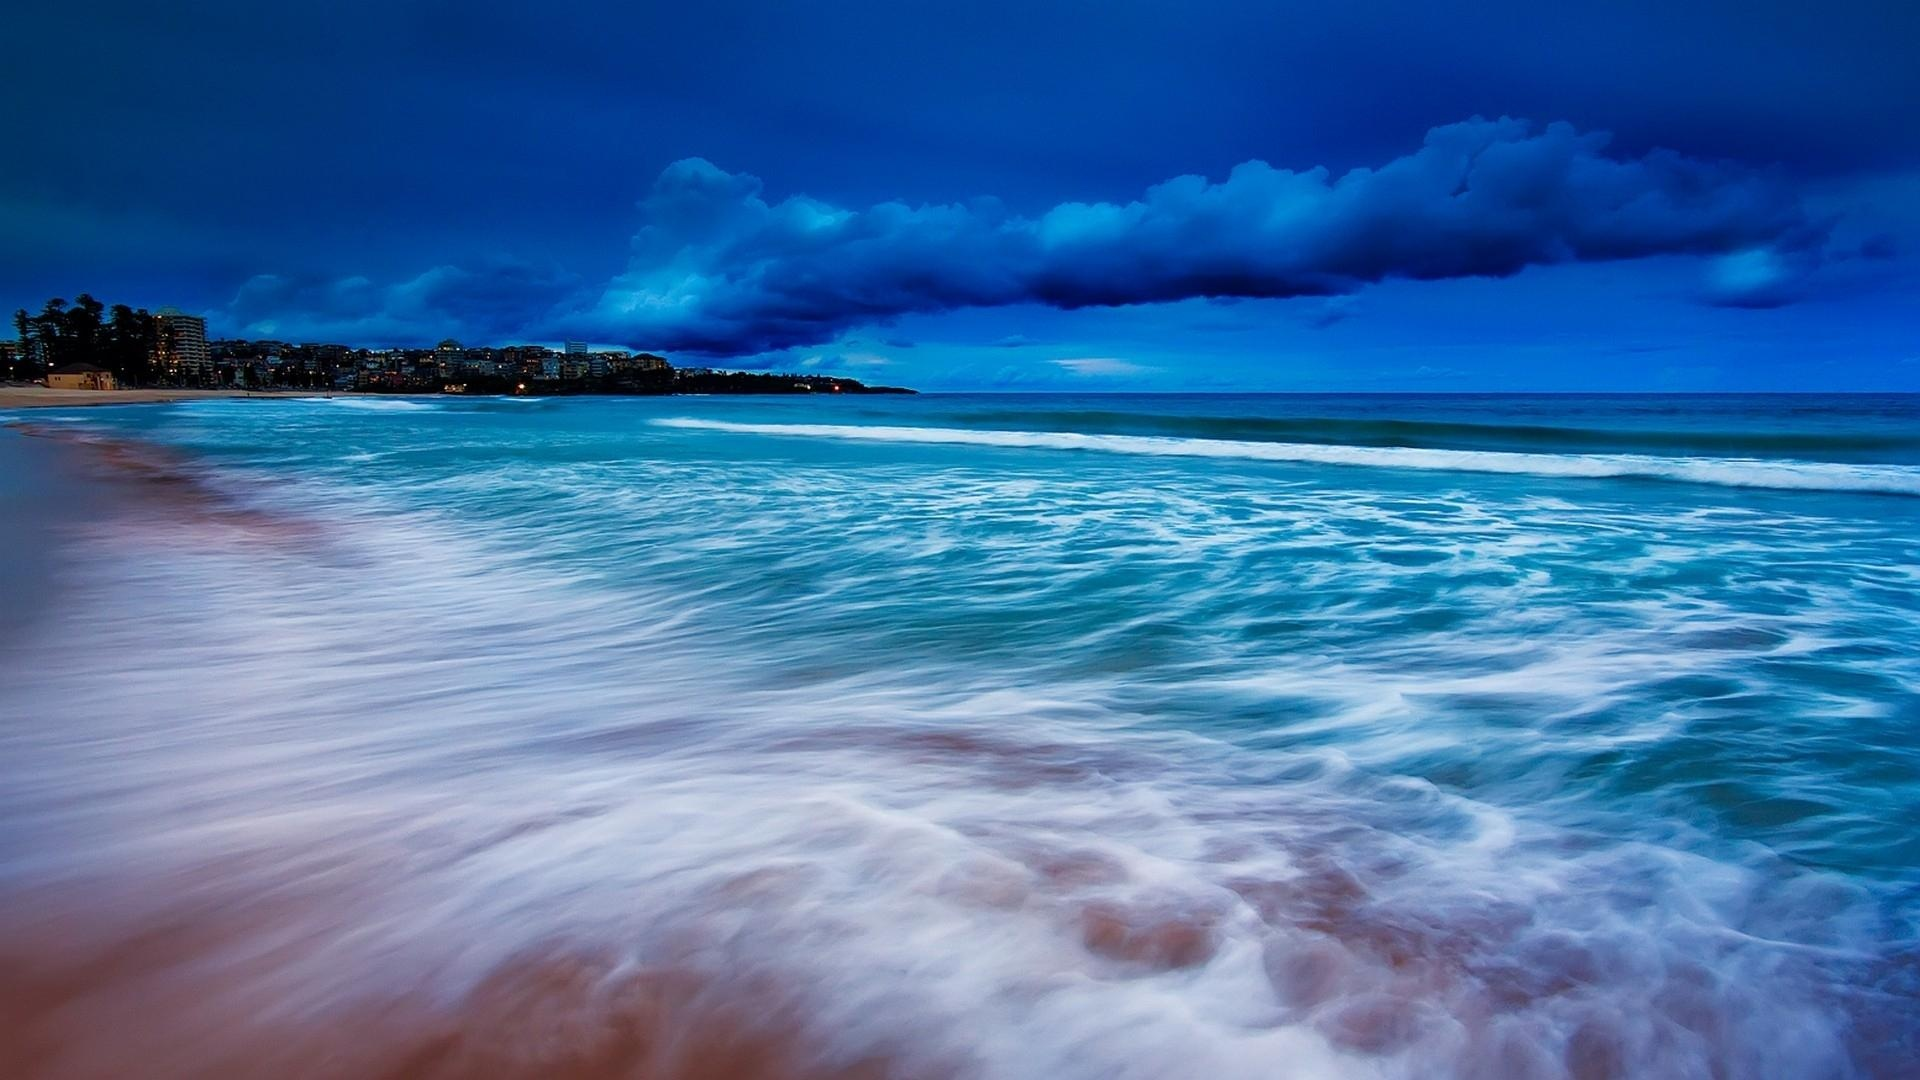
\includegraphics[scale=0.4]{1.JPG}
    \end{table}
\subsection{应用聚类分析将数据分组}
\subsubsection{数学模型}
K-Means 聚类分析:使用5.1.2中已经处理好的数据代表每一个企业。将每
个企业单独分为一组,随机选定其中的两个企业,使用欧氏距离计算两个企业与
其他全部企业的距离,针对两个企业,分别选择距离它们最近的其他企业,形成
两组包含两个企业的小组;对两个小组计算中心位置,使用中心位置坐标代表两
组数据的值,通过计算中心位置坐标值与其他企业的距离,找出距离两组数据最
近的企业点,重复上述做法,直到符合迭代停止的步骤。\par
数学模型如下:
\begin{enumerate}[i]
    \item 欧式距离公式:$ d_{ij} = \sqrt{(s_i-q_i)^2+(s_i-q_j)^2+(s_i-q_j)^2}$,其中$ i,j = 1,2,3\cdots123$。
    \item  本文将企业按照信誉等级分为三类,在此基础下,针对每一等级将企业分
    为前景良好值得投资与效益较差两类,使用三次 K-Means 聚类对数据进行分
    组,在聚类时k值取2。
    \item 聚类分析目标:由于需将数据划分为两组,假设最终分类的两组为$T_1$ 和$T_2$ ,
    每组数据中心为$t_1$和$t_2$。则有目标函数$min\sum_{s\in T_i}|s-t_i|^2$,其中$i =1,2$,数据中也称为质心,表达式为
    $t_i = \frac{1}{|T_i|}\sum_{S\in T_i} S$,其中$i = 1,2$。
    \item \[f_{(x,y) = }
    \begin{cases}
        x + y; & x > 10,y < 10\\
        2x + 4y; & x < 10, y < 10\\
        4x + 3y; & x < 10 ,y > 10 \\
        x + 22y; & x > 10,y > 10;
    \end{cases}\]
\end{enumerate}
    参考了\cite{ref1}
\begin{thebibliography}{99}  
    \bibitem{ref1}Zheng L, Wang S, Tian L, et al., Query-adaptive late fusion for image search and person re-identification, Proceedings of the IEEE Conference on Computer Vision and Pattern Recognition, 2015: 1741-1750.  
    \bibitem{ref2}Arandjelović R, Zisserman A, Three things everyone should know to improve object retrieval, Computer Vision and Pattern Recognition (CVPR), 2012 IEEE Conference on, IEEE, 2012: 2911-2918.  
    \bibitem{ref3}Lowe D G. Distinctive image features from scale-invariant keypoints, International journal of computer vision, 2004, 60(2): 91-110.  
    \bibitem{ref4}Philbin J, Chum O, Isard M, et al. Lost in quantization: Improving particular object retrieval in large scale image databases, Computer Vision and Pattern Recognition, 2008. CVPR 2008, IEEE Conference on, IEEE, 2008: 1-8.  
    \end{thebibliography}
\end{document}